\chapter{Problem statement}
\label{chap:problem-statement}

In order to have a good understanding of what the true meaning and problem of overproduction is, it is important to first of all define what \textit{reactive programming} is, what its relation to other programming patterns is and how this paradigm is implemented in the \textit{Reactive Extensions} API, which will be used throughout this thesis.

In order to understand these fundamental principles, this chapter starts off with defining what reactive programming is, as it is described in the literature. Since this paradigm forms the basis of this whole thesis, it is important to establish the notion of reactiveness first.

Then the Reactive Extensions API is discussed. It is the context in which overproduction occurs as well as the basis of the tools we will be using to solve this problem. Since this API is not yet considered to be common knowledge and since not much literature is based on it, we will start from the very basics and discuss all the concepts necessary for this thesis.

At the end of this chapter the overproduction problem is introduces in further detail, as well as related work that already provides solutions to this problem.

\section{Reactive Programming}
\label{sec:reactive-programming}
Currently one of the most difficult problems in computer science is handling big amounts of data. No longer are applications bound to the closed world of a single machine and a relational database. Applications these days have access to the whole World Wide Web, exist of large clusters of machines, work with data ranged from SQL-style relational databases to key-value pointer based databases, as well as binary data such as images, audio and video. Also the speed in which data is handled varies from `once a month' to `every millisecond'.

These changes in how applications need to perform require new ways of handling data. No longer is it feasible to load a whole database table into memory for further processing, nor can we permit ourself to wait for all data to be downloaded before we start processing it. Instead we require systems and concepts that are able to handle data right as it gets available to the application, without further delay, preferably in an asynchronous way and without blocking other processes or waiting for all data to have arrived. \cite{meijer2012-YMIAD}

An interesting part of the solution to these problems is Reactive Programming. This term is described by Albert Benveniste and G\'erard Berry in ``\textit{Real time programming: special purpose or general purpose languages}'' \cite{berry1991-Reactive} as he makes a distinction between \textit{interactive} and \textit{reactive} programs:

\begin{quote}
``\textit{Interactive programs} interact at their own speed with users or with other programs; from a user point of view, a time-sharing system is interactive. \textit{Reactive programs} also maintain a continuous interaction with their environment, but \textbf{at a speed which is determined by the environment}, not by the program itself.''
\end{quote}

Reactive programs `observe' events that occur in their environment and react to them as specified by the program. These events can vary from large amounts of data coming in over a network connection or from a database, to mouse moves or other kinds of UI events and from low-latency sensor streams to high-latency calls to web services.

Also notice that Benveniste and Berry explicitly emphasize that that reactive programs run at a speed which is determined by the environment. This means that the producer (which is part of the environment) is in charge of sending data to the consumer. Therefore the consumer (the program) cannot \emph{ask} for new data, it can only \emph{react} to the data that has been sent by the producer. This relationship between producer and consumer is often referred to as \textit{push based behavior}.

A classic example of push based behavior is a mouse pointer moving over the screen. Every time the pointer is moved, it will \emph{push} its new coordinates to the screen, for it to drawn in the new position. From its point of view, the screen \emph{reacts} to the new coordinates being received by the mouse pointer.

This push based behavior is in contrast with the relation between producer and consumer in an interactive program. Here, according to Benveniste and Berry, the consumer (program) interacts on its own speed with its environment. The consumer will determine the speed at which data is transmitted from the outside by continuously asking for the next bit of data. After this is received, the consumer processes the data and then asks for the next piece. This kind of interaction between consumer and producer is often referred to as \textit{pull based behavior}.

One example of a simple interactive program is a foreach-loop iterating over a collection of elements. As long as there are more elements in the collection, it will ask for the next one, process it according to the loop's body and then ask for the next element.

\section{Reactive Extensions}
There have been many attempts to fit the philosophy of reactive programming into libraries, APIs or even languages \cite{ReactiveX, meijer2015-Dart, Reactive-Streams, Akka, Elm, RxMobile}. In this section, we will briefly discuss some of the features of one of these libraries, namely Reactive Extensions (a.k.a. Rx). This project started at Microsoft with an implementation in C\# \cite{meijer2010-Observable} (Rx.Net), was later ported to Java, Scala, Groovy, Kotlin, JavaScript, Swift and many other languages by the open source community \cite{ReactiveX}.

However, these translations have deviated a lot from the original implementation. Most remarkable is that some of them are not even purely `reactive' anymore \cite{meijer2014-Derivation}. Given these deviations from the original paradigm and the state of complexity of these implementations, we decided to use a reference implementation of the original Rx that has recently been written in Scala by Erik Meijer called RxMobile \cite{RxMobile}, with the purpose of creating a light-weight implementation for developing mobile apps on Android. The following discussion and derivation of the API will however apply to both Reactive Extensions and RxMobile and in this section we will therefore refer to both as `Rx'.

\subsection{Core components}
\label{subsec:core-comps}
Rx is a library for composing asynchronous and event based (reactive) programs by using observable sequences. The core of Rx consists of two interfaces: \obs and \obv. The latter can subscribe and react to the events that are emitted by the former. An \obs can emit zero or more events (called \textit{onNext}) and has the possibility to terminate with an \textit{onCompleted} or \textit{onError} event. After either one of these terminal events is emitted, no more events can follow. Therefore the emission protocol can be summarized by the following regular expression: \code{onNext* (onError | onCompleted)?} \cite{MS2010-RxDesign}. When an \obv subscribes to an \obs,  it will return a \subs. With this object reference, one can later unsubscribe from the \obs and clean up potential resources.

\autoref{lst:obs-obv} shows these basic concepts of the \obs, \obv and \subs translated in Scala. Notice that here \subs is a superclass of \obv. Therefore there is no need for the \obs to return a \subs when an \obv subscribes to it. It will however return a \subs when another variant of \code{subscribe} is used, where for example a lambda expression is expected.

\begin{minipage}{\linewidth}
\begin{lstlisting}[style=ScalaStyle, caption={Observable, Observer and Subscription}, label={lst:obs-obv}]
trait Observable[T] {
    def subscribe(observer: Observer[T]): Unit
    def subscribe(onNext: T $\Rightarrow$ Unit): Subscription
    // other variants of subscribe
}

trait Observer[T] extends Subscription {
    def onNext(t: T): Unit
    def onError(e: Throwable): Unit
    def onCompleted(): Unit
}

trait Subscription {
    def isUnsubscribed(): Boolean
    def unsubscribe(): Unit
}
\end{lstlisting}
\end{minipage}

Creating an \obs is done by the \code{Observable.create(Observer $\Rightarrow$ Unit): Observable} method, that takes a lambda expression of type \code{Observer $\Rightarrow$ Unit} and returns an \obs. The input lambda is then used in the implementation of \code{subscribe}, when a \emph{real} \obv is provided. The \obv can be created by supplying it three lambda expressions, one for each kind of event.

\autoref{lst:create-sub-obs} provides a simple example of how both an \obs and \obv are created and used in practice. Here the function in \code{Observable.create} causes the \obs to emit three values and complete afterwards. Notice that these are only emitted after line~\ref{line:subscribe} is executed, when the \obv is subscribed to the \obs. If no one will subscribe, the values will never be produced nor emitted!

\begin{minipage}{\linewidth}
\begin{lstlisting}[style=ScalaStyle, caption={Creating and subscribing to an \obs}, label={lst:create-sub-obs}]
val xs: Observable[Int] $=$ Observable.create((obv: Observer[Int]) $\Rightarrow$ {
    obv.onNext(1)
    obv.onNext(2)
    obv.onNext(3)
    obv.onCompleted()
})
val observer: Observer[Int] $=$ Observer(
    (x: Int) $\Rightarrow$ print(x + " "),
    (e: Throwable) $\Rightarrow$ print(e),
    () $\Rightarrow$ print("completed"))

xs.subscribe(observer) |\label{line:subscribe}|

// result: 1 2 3 completed
\end{lstlisting}
\end{minipage}

Using \code{Observable.create} is a very powerful tool to create an \obs. Many other methods can be derived from it. For example, the \obs in \autoref{lst:create-sub-obs} is often written as \code{Observable.apply(1, 2, 3)}\footnote{In Scala this can be shortened to \code{Observable(1, 2, 3)}. Explicitly writing \code{.apply} is only done for later referral.}. This way of writing is not only more concise and conveys what the true meaning of this expression is in a better way, but it is also exactly the same, since \code{Observable.apply} is implemented in terms of \code{Observable.create}. In fact, all methods that are defined on \obs can be implemented using \code{Observable.create}!

\subsection{Derivation of \obs and \obv}
\label{subsec:derivation}
In 1994, the book `\textit{Design Patterns: Elements of Reusable Object-Oriented Software}' by the \textit{Gang of Four} was published \cite{gamma1994-DesignPatternsGOF}. This book explored the capabilities and pitfalls of object oriented programming and contained an overview of 23 classical software design patterns. Also, the book described the relationships between these 23 design patterns.

One of these design patterns is called the \textit{Observer} pattern and forms the basis of the \obs and \obv interfaces described in the previous section. Even though the Gang of Four did identify a lot of relations between the different design patterns, it failed to identify any relation between the Observer pattern and any other pattern, except for the Mediator pattern.

\begin{figure}[H]
	\begin{center}
		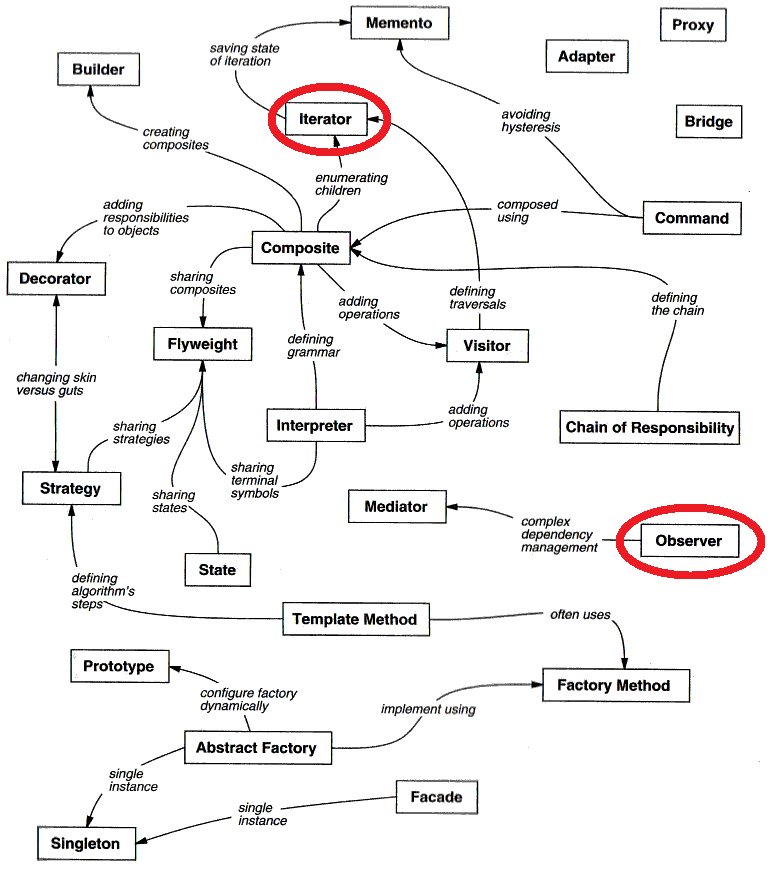
\includegraphics[width=0.48\textwidth]{figures/DesignPatternRelationships_bew.png}
	\end{center}
	\label{fig:designPatternRelationships}
	\caption{Relations between design patterns according to \cite{gamma1994-DesignPatternsGOF}}
\end{figure}

In 2010, Erik Meijer published a short paper called `\textit{Subject/Observer is Dual to Iterator}' \cite{meijer2010-Observable}, where he described a mathematical relationship between the Observer pattern and the Iterator pattern based on categorical duality. The paper shows that instances of the Observer pattern can be viewed as push-based collections, rather than the pull-based collections that result from the Iterator pattern. For later parts of this thesis, it is important to understand the mathematical basis of this relationship between the \obs and \obv interfaces in Rx and the \ieb and \ier interfaces in the Iterator pattern\footnote{For the purpose of the upcoming derivation we have chosen the C\# naming conventions of the Iterator pattern. In other programming languages these interfaces are respectively known as \code{Iterable} and \code{Iterator}.} (see \autoref{lst:itb-itr}).

In most common languages \ieb forms the basis of the Collections API. It has only one method \code{getEnumerator} that returns the \ier to iterate over the elements in the collection. The \ier interface on the other hand contains two methods to be implemented: \code{moveNext} and \code{current}. The former performs a side effect by moving a pointer to the next element in the iteration and then returns a \code{Boolean} to indicate whether or not there was a next element. The latter is a pure function that just returns the element the pointer is currently pointing to. Notice that the \code{moveNext} method can throw an exception rather than returning \code{false} in case an error occurs.

Besides providing these two methods, \ier in \autoref{lst:itb-itr} also extends the \id interface. This interface is meant to signal to the \ieb that no more elements will be pulled and that it can `start collaborating' with the garbage collector to clean up resources. The real meaning of \ier extending \id however, is that \code{getEnumerator} not only returns an \ier, but also returns something that is disposable. The \id interface is therefore not really part of \ier but rather a part of what \code{getEnumerator} returns \cite{E2E-Rx}. For now we will consider \id to be a silent bystander that is will be ignored in the derivation.

\begin{minipage}{\linewidth}
\begin{lstlisting}[style=ScalaStyle, caption={\ieb and \ier interfaces}, label={lst:itb-itr}]
trait IEnumerable[T] {
    def getEnumerator(): IEnumerator[T]
}
trait IEnumerator[T] extends IDisposable {
    def moveNext(): Boolean // throws Exception
    def current: T
}
trait IDisplosable {
    def dispose(): Unit
}
\end{lstlisting}
\end{minipage}

These two interfaces together form the basis of all pull-based or interactive collections as described in \autoref{sec:reactive-programming}. The user asks for the next element and will (eventually) get one in case a next element can be produced. In the following we will transform these interfaces for pull-based collections into interfaces for push-based or reactive collection, where the user subscribes to a collection and receives data once it is produced. This derivation, as well as its conclusion that interactive and reactive collections are each other's dual, is based on some categorical transformations and are discussed in several papers, as well as several keynotes and Channel9 video's \cite{meijer2010-Observable, meijer2012-YMIAD, E2E-Rx, meijer2014-Duality-And-The-End-Of-Reactive}. This derivation, as well as some of the intermediate steps are important for later parts of this thesis.

The first step in this derivation is to rewrite the two methods in the \ier interface into a single method \code{getNext()}. Using the categorical \textit{coproduct} \cite{rydeheard1988-Category-Theory} we can combine these two methods and determine its type signature: \code{getNext()} can either fail with an exception or succeed with either an element or no element, resulting in the type signature \code{getNext(): Try[Option[T]]}. The new, intermediate, set of interfaces is shown in \autoref{lst:itb-itr-interm}.

\begin{minipage}{\linewidth}
\begin{lstlisting}[style=ScalaStyle, caption={\ier interface after applying coproduct}, label={lst:itb-itr-interm}]
trait IEnumerable[T] {
    def getEnumerator(): IEnumerator[T]
}
trait IEnumerator[T] {
    def getNext(): Try[Option[T]]
}
\end{lstlisting}
\end{minipage}

Since both interfaces now only have one single method, and given that the only purpose of \ieb is to produce an \ier, they can be written as a single lambda expression. An \ieb can be written as:

\begin{equation} \label{eq:itb}
\code{() $\Rightarrow$ (() $\Rightarrow$ Try[Option[T]])}
\end{equation}

Notice that applying \code{Unit} to the outer lambda yields another lambda expression, which corresponds to the type signature of \code{getNext} in \autoref{lst:itb-itr-interm}: \code{() $\Rightarrow$ Try[Option[T]]}.

The next step in this transformation is to dualize \cite{rydeheard1988-Category-Theory} lambda~expression~\ref{eq:itb}. A very informal way of describing duality is to flip all the arrows and rewrite the lambda expression. For example, the duality of $f :: A \rightarrow B$ is $\bar{f} :: A \leftarrow B \equiv B \rightarrow A$. In the same way, we can apply this to lambda~expression~\ref{eq:itb}, resulting in

\begin{equation} \label{eq:obs}
\code{(Try[Option[T]] $\Rightarrow$ ()) $\Rightarrow$ ()}
\end{equation}

This lambda expression takes a lambda from \code{Try[Option[T]]} to \code{Unit}, and returns \code{Unit}.

We can now put this lambda expression back into context by splitting it into two interfaces. The inner lambda \code{Try[Option[T]] $\Rightarrow$ ()} can be rewritten to an interface called \obv, which has one method \code{onNext(t: Try[Option[T]]): Unit}. This method can then be further rewritten into three separate methods by expanding the \code{Try[Option[T]]} type: \code{onNext(t: T): Unit}, \code{onError(e: Throwable): Unit} and \code{onCompleted(): Unit}. The outer lambda on the other hand translates to an interface called \obs, which has one method \code{subscribe(obv: Observer[T]): Unit}. Notice how these interfaces are completely identical to the ones presented in \autoref{lst:obs-obv}.

%So far the presence of \id has been ignored in this derivation. This interface can however be found in \autoref{lst:obs-obv}, renamed as \subs. \todo{Add a couple of words on the functionality of \id and \subs and how they are the same.}

So far, the presence of \id has been ignored in this whole derivation. The reason for that is that this interface is considered to be a \emph{second} thing that is returned by the \ieb, rather than a supertype of \ier. What therefore basically happened in the derivation is that we only dualized the enumerator\textit{ness} and left the disposable\textit{ness} out of the dualization process \cite{E2E-Rx}. Therefore the dualized \ier, now called \obv, still extends from \id, even though this only means that we pass \textit{two} arguments to the \code{Observable.subscribe(obv: Observer)}. Just as the \id was meant to signal to the \ieb that no more elements will be polled and that it can clean up its resources, now \id signals to the \obs that it should stop sending data to the \obv. Finally, \id is renamed to \subs and its method \code{dispose} is split into two methods \code{unsubscribe} and \code{isUnsubscribed}.

% really dualized the enumeratorNESS but not the disposableNESS
% \ieb returned \ier AND \id
% now we dualized the enumeratorNESS, \id remained, so we need to return \id in \obs instead of void
% so when we subscribe to an \obs with an \obv, we get back a \id to unsubscribe later

This derivation shows that interactive, pull-based collections are the mathematical dual of reactive, push-based collections. The \obs and \obv interfaces can directly be derived from the \ieb and \ier interfaces. Both sets of interfaces can therefore be considered to be collections. In other words: streaming data behaves exactly the same way as regular collections, such as arrays, lists and sets, except for them being push-based rather than pull-based \cite{meijer2012-YMIAD, meijer2010-Observable}. In the world of push-based collections one \emph{subscribes} to the stream in order to \emph{react} to the next element that is being send, whereas one \emph{asks} for the next element in a pull-based scenario.

\subsection{\obs as a monad}
\label{subsec:obs-monad}
As described in the previous section, \obs can also be written as lambda~expression~\ref{eq:obs}. A better look at this expression reveals that \obs is actually a special instance of the \textit{continuation monad}, which has the following type:

\begin{equation} \label{eq:cont}
\code{(S $\Rightarrow$ R) $\Rightarrow$ R}
\end{equation}

In the \obs lambda expression, \code{S} is equal to \code{Try[Option[T]]} and \code{R} is equal to \code{()} or \code{Unit}.

Given that \obs is just a special instance of the continuation monad, it automatically has the two operators that are defined on all monads:

\begin{minipage}{\linewidth}
\begin{lstlisting}[style=HaskellStyle, caption={\obs as monad}, label={lst:obs-monad}]
newtype Observable t = Obs { runObs :: (t -> ()) -> () }

instance Monad Observable where 
    return :: Try[Option[T]] -> Observable[T]
    return t = Obs (\c -> c t )

    (>>=) :: Observable[T] -> (Try[Option[T]] -> Observable[S]) -> Observable[S]
    (Obs f) >>= g = Obs (\c -> f (\a -> let (Obs b) = g a in b c))
\end{lstlisting}
\end{minipage}

In the Rx implementation, these operators are present as well. The \code{return} creates an \obs from a \code{Try[Option[T]]}, meaning that it accepts either an error, or an empty value, or a non-empty value. Therefore \code{return} is split into three operators \code{apply(t: T)}, \code{error(e: Throwable)} and \code{empty()}. Since an \obs can have multiple values, \code{apply} is overloaded to have more than one value. This overload was already shown in section~\ref{subsec:core-comps} The \code{(>>=)} operator is renamed to \code{flatMap} and also splits the \code{Try[Option[T]]} parameter into three separate parameters \cite{rx-api}. Besides that, since the \code{T $\Rightarrow$ Observable[S]} parameter is used most frequently, the \code{flatMap} operator is overloaded with only this parameter.

A simple example of using these monadic operators in Rx is shown in \autoref{lst:monad-in-rx}. On line~\ref{line:return} the overloaded \code{apply} is called, which lifts four values into the \obs. The \code{flatMap} operator on line~\ref{line:flatMap} doubles the number of elements by creating an \obs that emits the value as well as the square of the value.

\begin{minipage}{\linewidth}
\begin{lstlisting}[style=ScalaStyle, caption={Monad operators in Rx}, label={lst:monad-in-rx}]
Observable(1, 2, 3, 4) |\label{line:return}|
    .flatMap(x $\Rightarrow$ Observable(x, x * x)) |\label{line:flatMap}|
    .subscribe(x $\Rightarrow$ print(x + " "))

// result: 1 1 2 4 3 9 4 16
\end{lstlisting}
\end{minipage}

\subsection{Operators}
\label{subsec:operators}
In section~\ref{subsec:derivation} we concluded that both the Iterator pattern and the Observer pattern are collections, only separated by the difference between push-based and pull-based behavior. All other rules on collections do however apply to both of them. In regular pull-based collections many operators are defined to manipulate, transform, filter, fold or group elements. These operators can therefore also be applied to push-based collections. One of them, \code{flatMap} was already shown in the previous section. However, rather than iterating over the pull-based collection and applying a transformation to each element, these operators \emph{react} to data being emitted by applying their particular transformation or side effect and passing the (transformed) data down to either a potential next operator or the \code{subscribe} method.

The Rx implementations of the \obs interface provide a wide variety of operators that apply all sorts of transformations to a data stream \cite{rx-api}. All operators are defined on \obs and will also return an \obs, making the API highly compositional. In order to understand how these operators work, we will look at some basic examples. Other, more advanced operators will be discussed in section~\ref{subsec:avoiding-overproduction}.

\paragraph{Filter}To select only those elements that satisfy a certain predicate, the operator \code{filter(p: T $\Rightarrow$ Boolean): Observable[T]} is used. Every time an element is received by this operator, the predicate \code{p} will be applied. If the element satisfies the predicate, it is passed downstream; otherwise the element will be discarded. \autoref{lst:operators-obs} shows in line~\ref{line:filter} how to select the odd numbers in a stream of integers by supplying a predicate.

\paragraph{Map}To transform one stream of data into another, the \code{map(f: T $\Rightarrow$ S): Observable[S]} is used. Each time an element (which is of type \code{T}) is received by this operator, the function \code{f} is applied to this element, yielding a new element of type \code{S}. This new element is then passed to down the stream. In \autoref{lst:operators-obs} the \code{map} operator is first applied in line~\ref{line:map} to the stream of filtered elements with a function that doubles the input.

\paragraph{Scan}Most operators do not allow for any form of internal state. They do not keep track of previous elements. An operator that can take the previous elements into account is \code{scan(seed: S)(acc: (S, T) => S): Observable[S]}. To this operator first of all a seed is supplied, which is the internal state of the operator before any value is received. Once an element is received, it will apply its internal state, together with that element to the accumulator function \code{acc} and produce an element to be emitted. This emitted value is also the new internal state of the operator. \autoref{lst:operators-obs} has a \code{scan} operator in line~\ref{line:scan} that takes the sum of all integers it receives and uses a \code{seed = 0}.

\paragraph{Drop}The \code{scan} operator is often used together with \code{drop(n: Int): Observable[T]}, which discards the first \code{n} elements and forwards all elements after that. The combination with the \code{scan} operator is used to prevent the seed value from being emitted further downstream, as is shown in \autoref{lst:operators-obs} line~\ref{line:drop}.

\paragraph{Take}Whereas \code{drop} discards the first \code{n} elements, \code{take(n: Int): Observable[T]} is used to only propagate the first \code{n} elements and discard all elements that come after that. In practice this means that the stream is terminated early with a call to \code{Observer.onCompleted()}. \autoref{lst:operators-obs} shows how \code{take} is used to only propagate the first and the second element and discard the third.

\begin{minipage}{\linewidth}
\begin{lstlisting}[style=ScalaStyle, caption={Operators on \obs}, label={lst:operators-obs}, columns=fixed]
Observable(1, 2, 3, 4, 5)		// emits:    1, 2, 3, 4,  5
    .filter(x $\Rightarrow$ x $\%$ 2 $==$ 1)			// emits:    1,    3,     5 |\label{line:filter}|
    .map(x $\Rightarrow$ x * 2)			// emits:    2,    6,    10 |\label{line:map}|
    .scan(0)((sum, x) => sum + x)	// emits: 0, 2,    8,    18 |\label{line:scan}|
    .drop(1)				// emits:    2,    8,    18 |\label{line:drop}|
    .take(2)				// emits:    2,    8 |\label{line:take}|
    .subscribe(x $\Rightarrow$ println(x))
\end{lstlisting}
\end{minipage}

Just as the interactive collections, Rx has defined its operators in a way that composition of operators is very easy. In this way, simple operators can be chained in order to create the complex behavior that is often desired. There are many more operators defined on \obs, which are not mentioned in this section. For a full overview, we refer to the documentation on the Rx websites \cite{ReactiveX, rx-api, Rx.Net}.

\subsection{Different kinds of streams}
\label{subsec:stream-kinds}
There are many kinds of observable streams that can all be implemented using Rx. For example, a clock or a timer is basically a stream of `ticks' that emits an element every time unit and therefore has a constant speed. A stream of keyboard events on the other hand emits an element every time a key is pressed and therefore most likely has a very irregular speed. A data stream can also be the result of a database query or a network call. In these instances it might take a certain amount of time before the first result is emitted, but every other result is received almost immediately after the first result appeared.

%\subsubsection*{Finite vs. infinite}
Some of these data streams, like the database query, are finite and will at a certain time in the future call \code{onCompleted}. Others, like the clock, will keep producing next elements forever, be it at a regular pace or quite irregular, like the keyboard. This kind of stream will never call \code{onCompleted}, but still may terminate with an error by calling \code{onError}.

%There exist many operators in Rx to control these particular cases. Infinite streams can be limited by using operators like \code{take(n: Int)} (see section~\ref{subsec:operators}), \code{takeUntil(predicate: T $\Rightarrow$ Boolean)} and \code{takeWhile(predicate: T $\Rightarrow$ Boolean)} that propagate all elements until or while a certain predicate is satisfied. Streams that terminate with an error can be resumed by operators like \code{retry()} or \code{onErrorResumeNext(resume: Throwable $\Rightarrow$ Observable[T])}, which respectively resubscribe to the same \obs or subscribe to another \obs.

%\subsubsection*{Hot vs. cold}
One other difference between certain streams is what happens when one subscribes multiple times to the same stream. Clocks or keyboard events, like broadcasters, emit values whether or not anyone is subscribed. If no one is subscribed, the events are still produced, but are immediately discarded. On the other hand, if multiple observers subscribe to the same stream, they will all receive the same events. This kind of stream is referred to as a \textit{hot} stream.

Some streams, like the \code{Observable(1, 2, 3, 4)} in section~\ref{subsec:core-comps}~and~\ref{subsec:obs-monad} or the database query, are not considered to be broadcasters. This kind of stream will create a new instance of itself every time an \obv subscribes to it. A second subscriber therefore receives the same result as a first subscriber, even though the second subscribes much later than the first one. This kind of stream is referred to as a \textit{cold} stream.

%A hot stream can be converted to a cold stream by sharing a single subscription with all observers. This can be done by operators like \code{share()} and \code{publish(f: Observable[T] $\Rightarrow$ Observable[S])}.

Notice that even though these differences do exist, they are not reflected in they type of the \obs. It is therefore always good to be careful with these distinctions and not to make any assumptions on streams being hot, cold, finite, infinite or error prone.

\subsection{Subjects}
A \subj can be viewed as a bridge between the \obv and the \obs. It can be subscribed to like an \obs, but can also observe another stream like an \obv. This is a very powerful tool that is often used as a starting point for a stream. Every time a certain event happens outside the context of the \subj, its \obv part can be called using the three methods. It will then process these events in its \obs part and propagate them down the stream.

A \subj can also be used to convert a cold stream into a hot stream. For this, a cold \obs is subscribed to the \subj. Because of this subscription, the cold \obs will be triggered to start emitting its events. The observable part of the \subj then becomes a hot \obs.

A special instance of \subj is the \bsubj, which behaves like a normal \subj but additionally emits its most recent value (or a seed or default value if none has been emitted yet) immediately after an \obv is subscribed to it. This is often used in user interface components like a text field to signal a certain initial state.

\section{Fast producers, slow consumers}
In the previous section we discussed that a reactive collection is equivalent to any interactive collection: it obeys the same rules and the same operators (like \code{map} and \code{filter}) can be defined. One difference however is that a reactive collection is push-based, whereas an interactive collection is pull-based. Rather than the consumer being in charge, asking for the next value, here the producer is in charge and \emph{it} decides when to emit a next value. The consumer just has to listen and can only react to the elements emitted by the producer. This is conform the definition of a reactive collection in section~\ref{sec:reactive-programming}: ``\textit{Reactive programs maintain a continuous interaction with their environment, but at a speed which is determined by the environment, not by the program itself.}''.

A risk that arises from allowing the producer to be in charge occurs when the consumer cannot keep up with the rate in which the producer is producing the data. This gives rise to the problem of what to do with the growing accumulation of unconsumed data.

A classic example of overproducing observables is the \code{zip} operator, which merges two (or more) streams by using a combiner function whenever both streams have produced an element. In this operator the problem occurs when one \obs always produces faster than the other. This is a problem, because \code{zip} cannot keep up with the rate in which the first \obs is producing, since the second \obs is much slower. The most common, but also slightly naive, implementation for this operator maintains an ever expending buffer of elements emitted by the first \obs to eventually combine them with the data emitted by the slower stream.

Ever expanding buffers is common answer to overproducing observables. A fast emitting stream is draining its data into a buffer and the much slower \obv eventually takes the data out of the buffer. The major problem with this solution (and thus with the implementation of \code{zip} as described above) is that the buffer will have to use an unwieldy amount of system resources.

\subsection{Avoiding overproduction}
\label{subsec:avoiding-congestion}
One way of dealing with overproducing observables is to simply avoid the problem and take proactive measures whenever it is expected happen. In the following we will discuss several ways to reduce the amount of data by using standard operators that are defined on the \obs interface. For this we distinguish two types of operators: lossy and lossless operators \cite{Backpressure-Explained}.

\subsubsection{Lossy operators}
One set of operators avoids the problem in a lossy way, meaning that some of the emitted data will be dropped.

\paragraph{Throttling} The \code{throttle(interval: Duration)} operator only propagates the first element that is received in a particular interval. All other elements are discarded. Once has finished, a new interval starts immediately, in which again the first received element is propagated and all other elements are discarded.

\paragraph{Sample} Rather than propagating the first element and discarding all others, the \code{sample(interval: Duration)} operator is used to discard all elements except for the last one that is received in a certain \code{interval}. This operator can for example be used when someone only wants to receive the data from a stock ticker every 5 seconds, without the need to process every value that comes in between.

\paragraph{Debounce} The operator \code{debounce(timespan: Duration)} will only propagate its received values after a certain \code{timespan} has passed without receiving an other value. When a value is received within the \code{timespan}, the previous value is discarded and the same process starts all over again with the newly received value. This operator is most commonly used in text fields within user interfaces, in order to avoid too much keystroke events being generated by a fast typing user. Rather than every keystroke being emitted, this operator will only yield the last keystroke after a particular \code{timespan}. Notice that in some versions of Rx this operator is also referred to as \code{throttleWithTimeout}.

With these operators many situations of potentially overproducing observables can be avoided by eliminating all the elements that do not really matter for a particular application.

\subsubsection{Loss-less operators}
Even though these lossy operators solve a large part of the problem, there are still as many cases left in which \emph{all} data that is send over a stream needs to be processed. For these kinds of use cases Rx provides so-called loss-less operators. These operators can buffer or group the data and emit collections of data, such that there are at least less elements to deal with.

\paragraph{Buffer} The \code{buffer} operator comes in a couple of different overloads. First of all, the \code{buffer(n: Int): Observable[List[T]]} operator, which receives data and groups it into lists of \code{n} elements. Once a list is filled (its size is \code{n}), it is emitted to downstream. Until then, the operator holds the data it receives. The \code{buffer} operator also comes in another form: \code{buffer(interval: Duration)}, which groups the data it receives within a certain interval into a single list. Finally there is \code{buffer[B](boundary: Observable[B])}, which groups the data it receives between two emissions of \code{boundary} into a single list.

\paragraph{Window} The drawback of a buffer is that it only propagates its received values once the buffer is filled, the boundary \obs fires or the interval is over. All the time in between no elements will be received by the observer or downstream operators. This already becomes clear from the return type: \code{Observable[List[T]]}. In order to accomplish the same behavior but with an \obs rather than a \code{List}, the \code{window} operator is included in Rx, having the same overloads as \code{buffer}. Instead of the list being emitted only once it is completely filled, the inner \obs is emitted as soon as the first element is received and is \emph{completed} once the size, interval or boundary requirement is met.

These operators form a first line of defense against overproduction. For streams where not all elements necessarily need to be processed (for instance the keyboard events on a text field), a lossy operator can be used. For streams where all emitted data is needed, a loss-less operator is the right solution. Besides that, for special occasions lossy and loss-less backpressure operators can be combined in order to create the optimal buffering strategy. This was discussed in some further detail in a conference talk at QCon by Ben Christensen \cite{christensen2014-RxServiceArchitecture}.

\subsection{Callstack blocking}
Another way of dealing with this problem is to block the callstack and with that `park' the thread on which the \obs is running. This directly slows down the producer and gives the consumer more time to process each element of the stream. Despite the fact that this approach goes against the `reactive' and `non-blocking' model of Rx, it can potentially be a viable option if the overproducing \obs runs on a thread that can safely be blocked.

This technique is currently not used in RxJava, but \emph{is} used in a particular implementation of the \code{zip} operator in RxMobile \cite{RxMobile}. Once either one of the streams emits a value, it is blocked until the other \obs has produced a value as well. In order to avoid blocking the upstream callstack completely, it is strongly recommended to switch each \obs to another thread or scheduler using the \code{observeOn} operator. With this only the callstack is blocked upto the start of this new thread or scheduler. Once the other stream has produced a value, the blocking of the first \obs sequence is removed and the \code{zip} operator waits until either one of the sources emits a next value.

\subsection{Reactive Streams}
Reactive Streams is an initiative \cite{Reactive-Streams} of a number of companies such as Netflix, Pivotal and Typesafe with the mission to \textit{provide a standard for asynchronous stream processing with non-blocking backpressure}. This collaboration resulted in an alternative API \cite{Reactive-Streams-API} for stream processing that is claimed to be capable of handling overproducing observables using backpressure.

This Reactive Streams API (see \autoref{lst:pub-sub}) looks fairly similar at first glance to the original API that was developed by Microsoft, but has some particular differences that have significant influence on the handling of backpressure. The \obs, renamed \code{Publisher}, looks the same: it still is parameterized over \code{T} and still has a \code{subscribe} method. The \obv, which was passed to the \code{subscribe} method, is replaced with a \code{Subscriber}, even though it is almost the same\footnote{The \code{onComplete} method in \autoref{lst:pub-sub} does not contain a typing error compared to \autoref{lst:obs-obv}. This is actually how the API is specified!}. It only adds an extra method \code{onSubscribe}, which is called right after the \code{Subscriber} is subscribed to the \code{Publisher}. This \code{onSubscribe} method requires an argument of type \code{Subscription}. This last interface contains two methods: \code{cancel}, which is similar to the \code{unsubscribe} method in \autoref{lst:obs-obv} and a new method \code{request(n: Long)}.

\begin{minipage}{\linewidth}
\begin{lstlisting}[style=ScalaStyle, caption={Publisher, Subscriber and Subscription}, label={lst:pub-sub}]
trait Publisher[T] {
    def subscribe(s: Subscriber[T]): Unit
}

trait Subscriber[T] {
    def onNext(t: T): Unit
    def onError(e: Throwable): Unit
    def onComplete(): Unit
    def onSubscribe(s: Subscription): Unit
}

trait Subscription {
    def cancel(): void
    def request(n: Long): Unit
}
\end{lstlisting}
\end{minipage}

This last method reveals the whole idea behind the Reactive Streams API, namely to let the \code{Subscriber} request a certain amount of elements from the \code{Publisher}. This way the \code{Subscriber} is in charge of how many elements it will receive eventually and the \code{Publisher} just has to send at most this amount of elements by calling the \code{onNext} method.

Taking a step back and evaluating the true meaning of what the Reactive Streams collaboration has come up with, results in the conclusion that this API is interactive rather than reactive, since it lets the consumer (\code{Subscriber}) be in charge of the rate at which data is sent to him. This is discussed in more detail in a conference talk at Lambda Jam 2014 by Erik Meijer \cite{meijer2014-Derivation}. Compared to the earlier discussed \ieb collections, it only adds the features of non-blocking and requesting more than one element (which is what the \ieb interface technically does) per request. We will discuss the consequences of this API in more detail in a later section.

\subsection{Reactive pull}
The ideas that sprout from the Reactive Streams initiative have been incorporated in the RxJava library. They kept the original naming conventions of \obs and \obv but added a couple of new methods to the latter: \code{request(n: Int)}, which signals to the \obs that it will be able to handle \code{n} new elements and \code{onStart()}, which performs the initial request from the \obv to the \obs. After the initial request is done, the \obs sends at most \code{n} elements to the \obv, which receives them in the \code{onNext} method. This is now the place where the \obv can call \code{request} again to receive more data.

We recognize these two methods from the Reactive Streams API, where \code{onStart()} was called \code{onSubscribe} and \code{request(n: Long)} was inside the \code{Subscription} interface. Making these slight modifications does not change the intention of the Reactive Streams API: it introduces a feature called \textit{reactive pull} in the \obv to manage the number of elements that are emitted by the upstream \obs.

Earlier versions of RxJava, who did not have this feature only had the ability to communicate upstream by calling the \code{unsubscribe} method. Recall that when an unsubscribe occurs, the \obs is basically signaled to stop emitting any data to the \obv. Besides unsubscribing there was no way in the standard Rx model to communicate upstream.

This feature from Reactive Streams allows the \obv to have some more control by \emph{pulling} from the data source (\obs) at its own pace. RxJava is set up in such a way that processing data under normal circumstances is still push based. Only when the \obv can't handle the speed in which data is sent, it will switch to this pull based model. Wrapping it up in this way, the problem of overproduction is not prevented or gone away but is rather moved up the chain of operators to a point where it can be handled better \cite{RxJava-Wiki-Backpressure}.

With this it limits the number of elements that are in a buffer within certain operators. Using this new feature, the earlier mentioned \code{zip} operator is implemented by using a small buffer for each \obs. It only requests items from one of these sources when there is room for more elements in its buffer. Once all buffers contain at least one element, the operator can remove an element from each buffer, zip these together and push them downstream. After that there is room for at least one extra element in all buffers, hence new requests are sent to the upstream.

Notice that the RxJava wiki \cite{RxJava-Wiki-Backpressure} points out that this method only works when all streams that are zipped together respond correctly to the \code{request()} method. This is \emph{not} a requirement for the normal \obs, but it is required for instances of \obs that are used in operators like \code{zip} that depend on reactive pull. RxJava therefore provides operators such as \code{onBackpressureBuffer} and \code{onBackpressureDrop} that respectively buffer and drop data that cannot be consumed immediately by the downstream \obv.

\subsection{Transmission Control Protocol}
A well known protocol from the Internet protocol suite is the Transmission Control Protocol (TCP), which offers reliable delivery of streams of data between applications communicating over an IP network \cite{tanenbaum2011-Computer-Networks}. In order to avoid having a sender to send data too fast for the TCP receiver to receive and process the data, it uses an end-to-end flow control protocol with a sliding window. The receiver specifies in the TCP header's \textit{Window Size} what amount of additional data it is willing to receive and buffer for the current connection. The sending host can only send at most that amount of data and has to wait for an acknowledgment and window update from the receiving host.

In case the sender receives a window size of 0, it obviously cannot send any data and instead starts a so called \textit{persist timer} that protects the TCP connection from a permanent deadlock. When this timer expires without the sender having received any new window sizes, it will send a small packet in order of the receiver to send a new acknowledgment containing a new window size.

The problem solved by this flow control protocol is in fact the same as overproducing observables discussed in this section. The solution presented by TCP is similar to \textit{reactive pull} and \textit{Reactive Streams} in the sense that they too advertise an `available buffer space message' to the \code{Producer} or \obs by calling the \code{request} method. The difference with TCP is that the earlier discussed solutions do not have the need for a persist timer since deadlock from lost window updates is not possible.

\todo{something more on this???}










































